% Author: Magdalen Berns

\chapter{The Eye}

\label{anatomy}
\lhead{\emph{The Eye}}

To develop technologies that image the retina, a full understanding
of the eye is necessary as well as a physical understanding of how it
processes light. The functioning of a normal healthy is explored and eye
dysfunction, pathology and injury is also detailed.

\section{A Normal, Healthy Eye}

The human eye is a complex biological system, which allows the brain to
form an image of its surroundings through the interpretation of
electromagnetic signals. \Fref{fig:eye_simple} shows a simple schematic
diagram of the layout of the eye. The structure of the eye is designed to
project a focused image onto the the back of the retina so the light rays
can be converted into electrical signals which are passed to the brain by
the optic nerve.

\begin{figure}[H]
\centering
  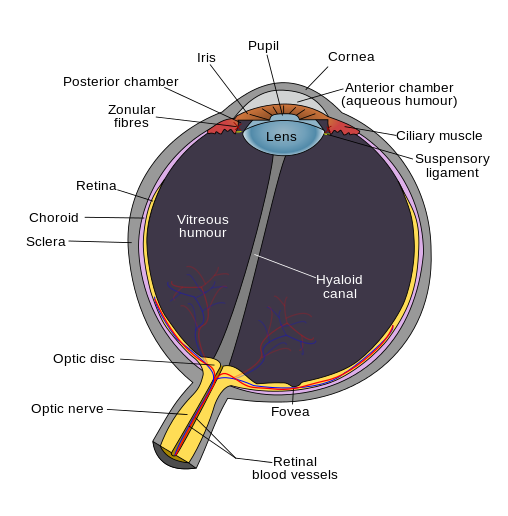
\includegraphics[width=8cm]{figures/schematic_diagram_of_the_human_eye}
\caption{A simple schematic diagram of the layout of the eye.\cite{wikiRhcastilhos}}
\label{fig:eye_simple}
\end{figure}

The cornea of the eye is a transparent layer around 0.6mm thick
which curves around the iris as well as the anterior
chamber.\cite{yaylali1997corneal,thoft1983x,patel1994refractive}
Its outermost surface is made of epithelial cells which are cyclically lost
and replenished.\cite{jester1999cellular,hassell2010molecular} The
reproduction of cells is facilitated in part by tear ducts, which serve
to moisten the eyes and remove harmful bacteria.\cite{holly1977tear}

With a mean refractive index of around 1.4 (about the same as water),
the cornea allows plenty of light to pass through. Incident light refracts
as in a convergent lens due to the convex shape of the cornea. Since
the refractive index of the air is different than that of the cornea, Snell's
Law of refraction models the path of the light ray through the
eye. \Eref{eq:refractive} gives Snell's Law of refraction for a light wave
passing through two different isotropic materials which have refractive indices
$n_1$ and $n_2$, respectively.

\begin{figure}[H]
\centering
  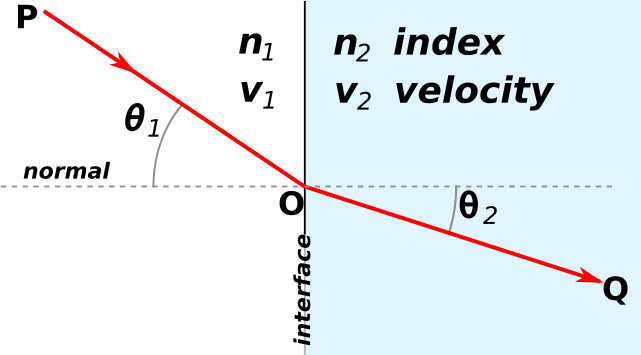
\includegraphics{figures/snells}
\caption{Snell's law for refraction at an interface where
             $n_1$\textless $n_2$.\cite{wikisnell}}
\label{fig:snell}
\end{figure}

The angle $\theta_1$ is between the normal to the interface ($n_1$ and $n_2$)
and the incident light ray and the angle $\theta_2$ is between the normal to
the interface ($n_2$ and $n_1$) and the transmitted light ray, as shown in
\fref{fig:snell}.

\begin{equation}
n_1\sin\theta_1=n_2\sin\theta_2
\label{eq:refractive}
\end{equation}

There is a small circular opening in the iris (the coloured section of
the eye) called the pupil, which has an aperture of around 7mm that
dilates to allow an appropriate amount of light to pass through
the lens onto the retina.\cite{krugman1964some} As a consequence of
this optical setup the pupil acts as a diffraction grating, which places a 
fundamental limitation on visual resolution. 

The angular resolution, $\theta$, of the focal point on the retina is limited by
the diameter, $D$, of the pupil and is directly proportional to the wavelength
of the diffracted light, $\lambda$, as expressed in the Rayleigh criterion
 \eref{eq:res_limit}.\cite{rayleigh1907dynamical}

\begin{equation}
\theta=\frac{1.22\lambda}{D}
\label{eq:res_limit}
\end{equation}

To find the optical resolution, the angular resolution must be multiplied by the
object's distance from the eye The maximum achievable resolution of the eye
corresponds  to $500\textrm{nm}$, using \eref{eq:res_limit} along with the diameter of
the pupil of 7mm in \eref{eq:eye_res} we can obtain a value for the angular
resolution of the eye, $\theta=87\times 10^{-6}$ radians.

\begin{equation}
\theta=\frac{1.22\times 500\textrm{nm}}{7\textrm{mm}}
\label{eq:eye_res}
\end{equation}

Following the initial refraction through the cornea, light is again refracted
through the lens to finely focus the image to a central point on the retina.
\Fref{fig:light_journey} illustrates the journey of light through the eye
onto the retina. The final image projected onto the retina is actually an
upside down projection of the original images. To counteract this, the
brain is conditioned to automatically flip the images so the image eventually
seen is right side up.

\begin{figure}[H]
\centering
  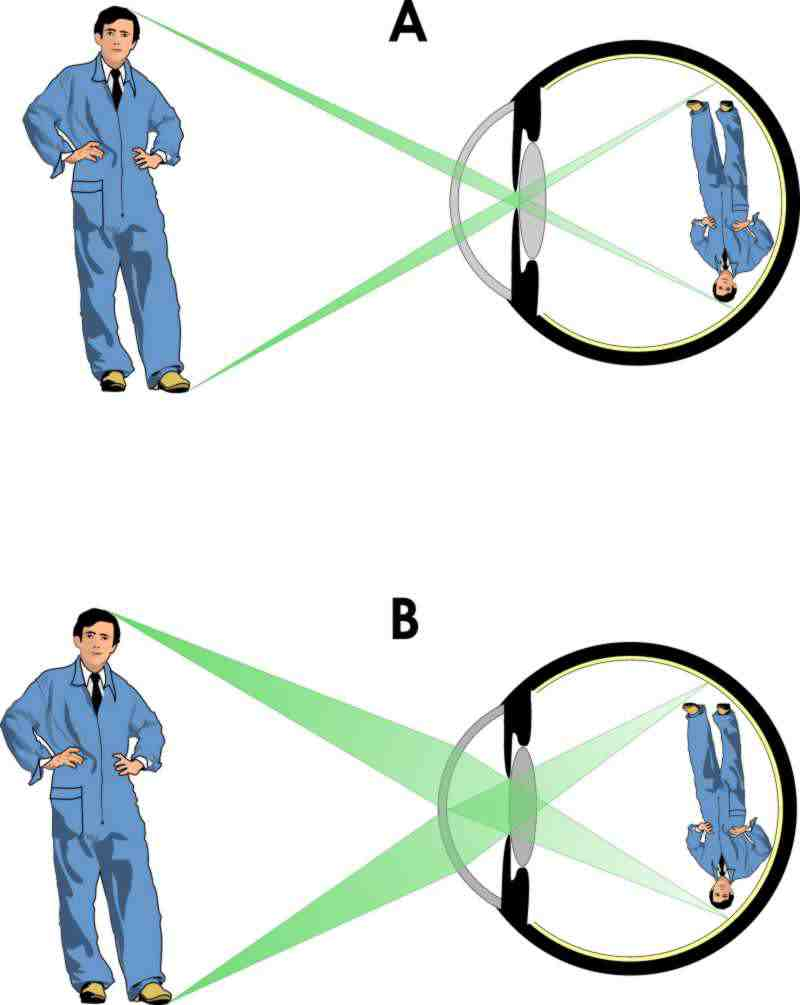
\includegraphics{figures/light_path}
\caption{(A) is an eye looking at a man through a pupil with his whole form in focus.
		The light only minimally disperses in front or behind the focal point
		on the retina. (B) shows the same situation, but with a dilated pupil.
		In this case, the image at the focal point on the retina is sharp but
		the clarity of the image is rapidly lost at points behind, or in front
		of the retinal focal point.}
\label{fig:light_journey}
\end{figure}

Focusing the image on the retina is important in obtaining clear images of
surrounding objects. Normal eyes are optically similar to a convex lens and
can be modelled using the lens maker's formula \eref{eq:lens_makers}
which relates the focal point of a lens to the distance of the object and
image from the lens centre, as is illustrated in \fref{fig:convergent_lens}.

\begin{equation}
\frac{1}{S_1} + \frac{1}{S_2} = \frac{1}{f}
\label{eq:lens_makers}
\end{equation}

\begin{figure}[H]
\centering
  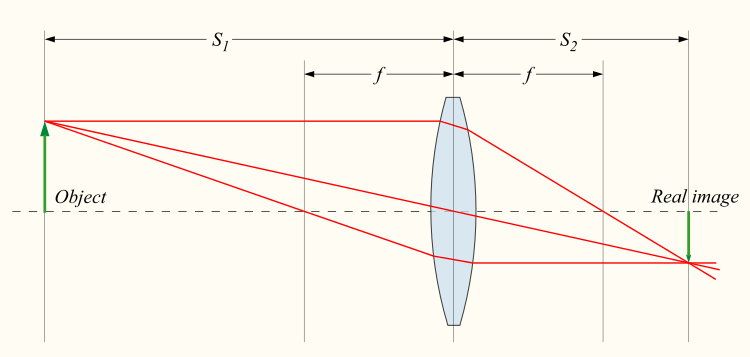
\includegraphics{figures/convergent_lens2}
\caption{The convex lens focuses the object (distance $S_1$ from the lens centre)
         and inverts this image (at a distance $S_2$ from the lens centre).
         \cite{greivenkamp2004field}}
\label{fig:convergent_lens}
\end{figure}

The lens is accommodated by a ciliary body of tissue which is made up of fibre and
muscle. The ciliary body secretes a fluid (aqueous humour) into a canal medically
known as scleral venous sinus, which channels fluids around the circumference of the
eye.\cite{bill1970effects,dvorak1934schlemm} The primary function of the aqueous
humour is to maintain intraocular pressure.

Another function of the ciliary body is to control the lens by contracting and relaxing the
ciliary body muscles. When the eye focuses on objects that are nearby, the ciliary body
muscles contract, causing the lens to flatten as a result of contractile forces. On the
other hand, if an  object is far away the light rays can be approximated as parallel to the
principal axis of the lens and the suspensory ligaments relax allowing the lens to return
to a normal curved shape.

\begin{figure}[H]
\centering
  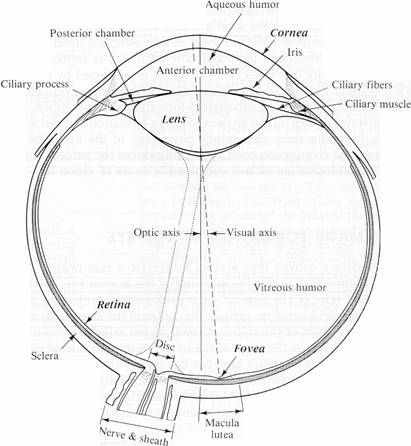
\includegraphics[width=8cm]{figures/eye_diagram}
\caption{A diagram of the eye showing of the visual
 	     and optic axis (indicated by the solid line), the cornea, the retina, the fovea
              and the visual axis (indicated by the dotted line).}
\label{fig:optic_axis}
\end{figure}

Unlike in the lens approximation where the light passed through air before forming an
image, the light leaving the lens must pass through a clear substance called the
vitreous chamber before arriving at the retina. Photons of light are refracted out of the
lens before they pass through a clear substance called the vitreous chamber and land
onto the retina, which is also transparent. A diagram indicating the optic axis and
visual axis is shown in \fref{fig:optic_axis} where the dotted line is the visual axis and
the solid line is the optic axis.

\begin{figure}[H]
\centering
  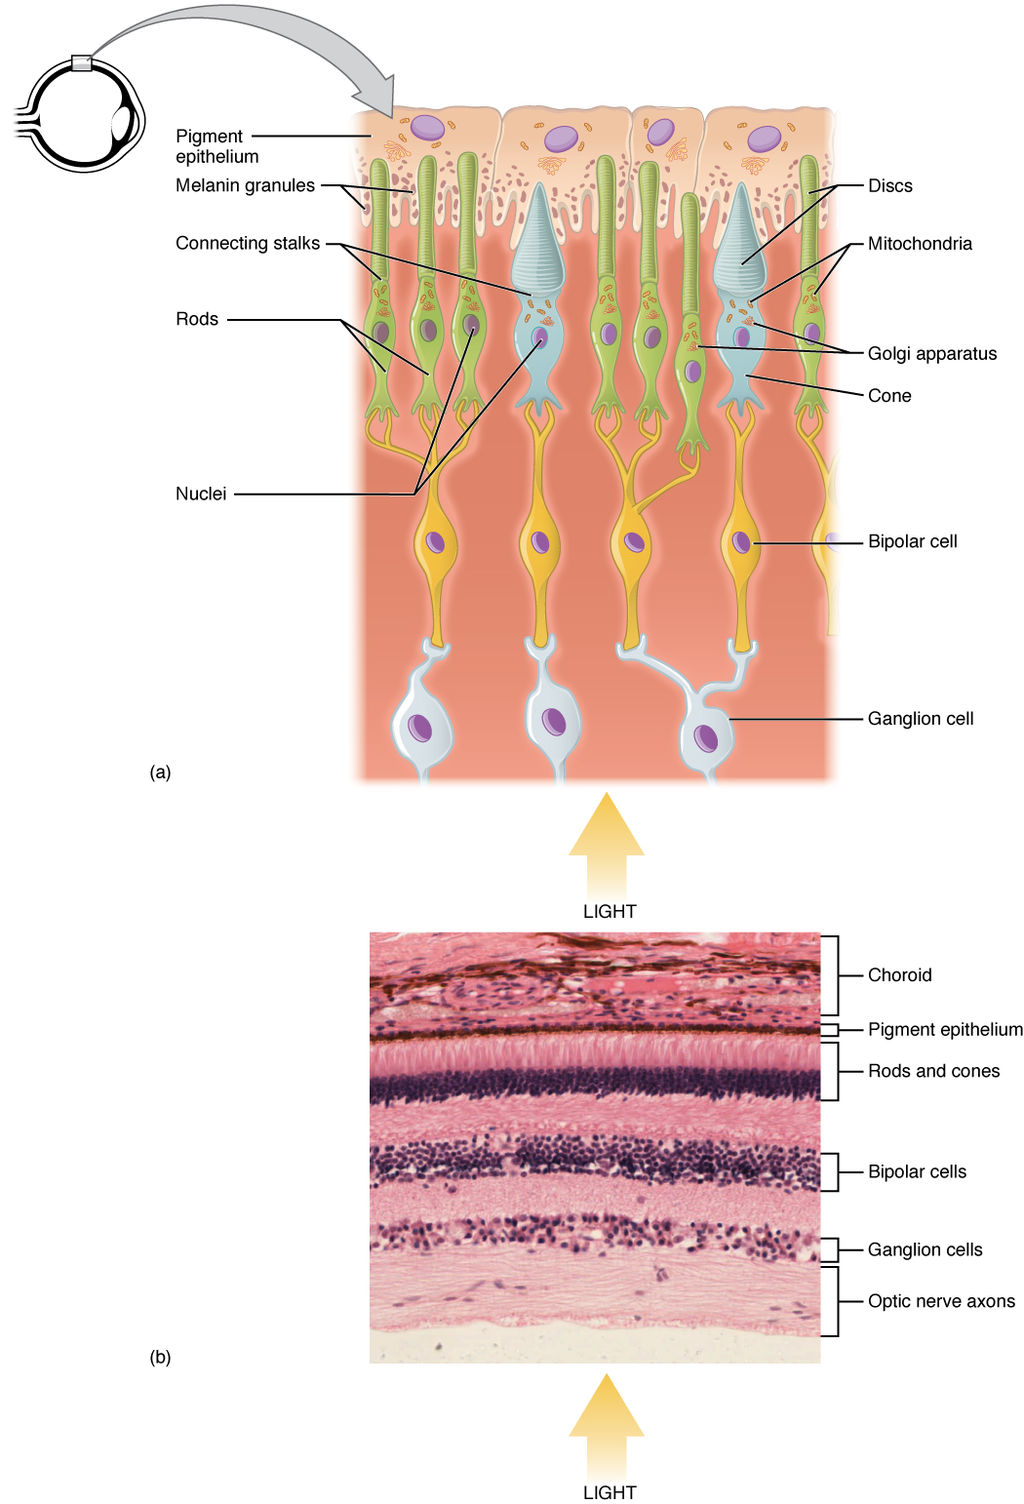
\includegraphics{figures/rods_and_cones}
\caption{A schematic diagram of the retina with the direction of light indicated
as being from the bottom upwards direction.}
\label{fig:retina}
\end{figure}

The retina is a membrane which covers the entire receptive field of
vision, and is part of the central nervous system.\cite{rogers1983neurite}
\Fref{fig:retina} shows a schematic overview of the retina. Just behind the
retina are ganglion cells, bipolar cells, cones and rods. These are supported
by pigment epithelium cells and the choroid - a vascular bed of tissues which
supply the retina with blood and removes toxins. \cite{lutty1996localization} 

There are around 0.7 to 1.5 million ganglion cells in a normal human retina.
\cite{curcio1990topography} Retinal ganglion cells are a form of neurons
and are integral in the transmission of electrical signals to the brain.
\cite{meyer1995characterization} Cones and rods are photoreceptors
that convert light into electrical signals which are transmitted to the
brain from the optic nerve, via bunches of ganglion nerves.

\begin{figure}[H]
\centering
  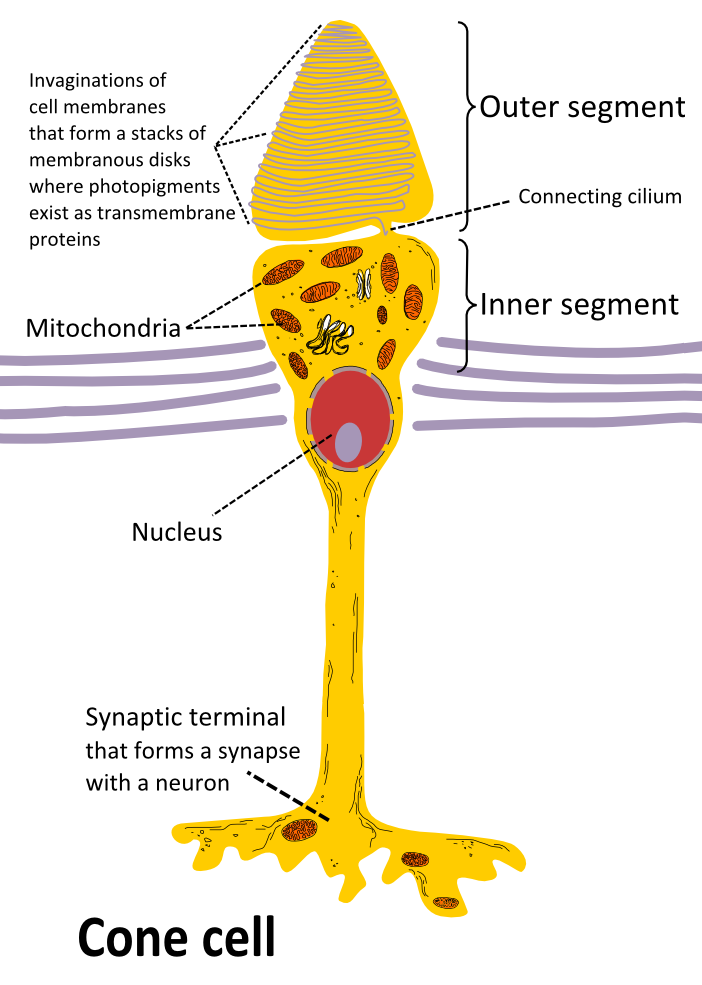
\includegraphics{cone_cell}
\caption{A schematic diagram of the cone cell showing the outer and inner
segments, nucleus and the synaptic terminal.\cite{wikicone}}
\label{fig:cone}
\end{figure}

Whilst cones are not particularly sensitive to light, they do aid visual
acuity by granting us colour vision (\fref{fig:cone} shows a schematic
diagram of the cone cell).\cite{bowmaker1980visual} Conversely, rods
which have a region of pigments around $1\mu{m}$, are particularly
sensitive, even to the pressure exerted by a single photon of light.
Rods tend to be located around the periphery of the receptive field to
maximise peripheral light collection.
\cite{liebman1964sensitive,baylor1979responses}

Most of the retinal cones are located around a circular trough in the
receptive field, called the fovea centralis which is located at the centre
of the macula.\cite{hendrickson1994primate}
\Fref{fig:rod_cone_density} is a graph of the density of cones and rods
against their angular distance from the fovea. The fovea is the most
sensitive part of the eye, which is why most cones are located directly
behind it. At the optic disc head there are no photoreceptors, this region
in the visual field is known as the blind spot.

\begin{figure}[H]
\centering
  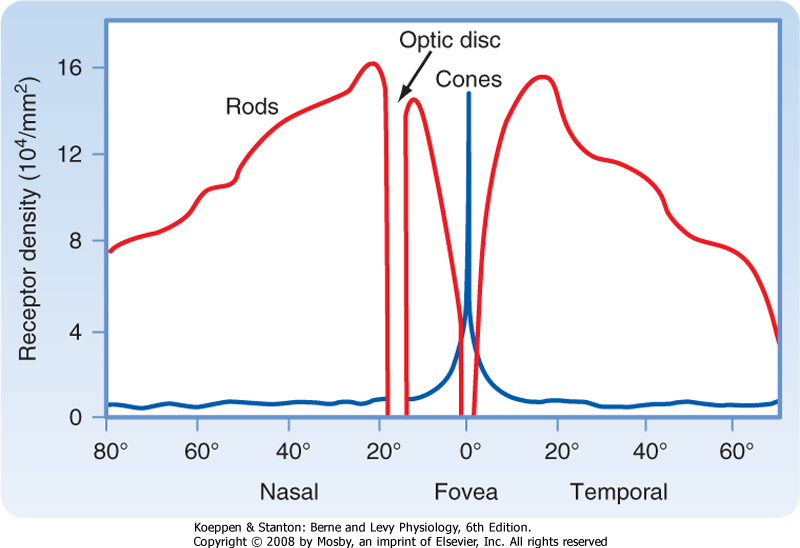
\includegraphics{rod_cone_density}
\caption{Plot of density of cones and rods against their angular distance from
the fovea. The cone density peak lies at the fovea, where there is an absence
of rods.}
\label{fig:rod_cone_density}
\end{figure}

The fovea has an apparent dip, because unlike the periphery, there are
no neurons situated behind it. Neurons are cells which process and
transmit electrical information. An extended nerve fibre known as an axon,
connects the cell body to the optic nerve, passing visual information to the
brain. As the photoreceptors (mainly cones) beneath the fovea are responsible
for the acuity and colour of the centre field of vision, axons would disturb the
tissue and result in a distorted visual field if they were beneath the fovea too
and this explains why there is a dip around this area of the macula.
 
 \begin{figure}[H]
\centering
  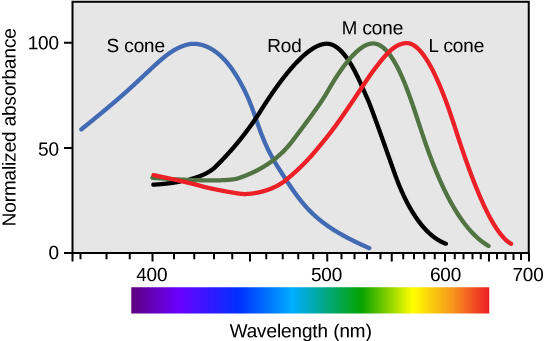
\includegraphics{wavelengths}
\caption{Normalised absorbance vs. wavelength, for cones of an average eye.\cite{wikicones}}
\label{fig:wavelengths}
\end{figure}

A healthy, normal eye is tuned to either red, green or blue light so that the
brain can interpret the full spectrum of colours. To illustrate how the
components of the eye detect different wavelengths of light,
\fref{fig:wavelengths} has been included. This shows normalised absorbance
against wavelength for S (blue), M (green) and L (red) cones as well as for
rods in an average human eye.  From \fref{fig:wavelengths} it can be seen
that the range of human visual spectrum of light lies roughly between 390nm
and 700nm.\cite{starr2010biology}.

\section{Dysfunction in the Eye}

Unlike an ordinary optical system there exists the added complication
of common irregularities in patient vision, such as myopia, astigmatism
or hyperopia. \Fref{fig:myop} demonstrates the optical effects of myopia,
a condition which occurs when the eyeball is shaped like a prolate oval.
\cite{saine2002ophthalmic} With myopia, light entering the eye is projected
in front of the retina instead of on its fovea, so although the lens will be
accommodated to focus nearby objects, difficulty arises when focusing on 
distant objects without the use of corrective lenses.

\begin{figure}[H]
\centering
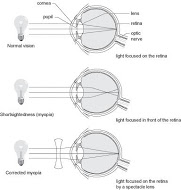
\includegraphics{figures/myopia}
\caption{An illustration of the visual effects of myopia and how it is corrected.}
\label{fig:myop}
\end{figure}

Conversely, when the eyeball is shaped like an oblate oval this can cause
hyperopia, a condition where light entering the eye is projected beyond the
retina so that it is difficult to focus on objects which are nearby without
corrective lenses.

Other deviations from the model shape of an iris, for example a conical
or oval-like shaped iris, can result in a condition called astigmatism.
Astigmatism is a condition which can distort visual perception in a myriad
of ways depending on the nature of the irregularity of the iris.

Two other common defects which do not relate to the shape of the iris are
presbyopia and \enquote{colour blindness}. As people age, ciliary muscles
accommodating the  lens weaken impairing their ability to focus on objects
which are close by, this is presbyopia. \cite{fisher1985ciliary}
\enquote{Colour blindness} is caused by the limited functionality of certain
cones which are sensitive to specific frequencies of light such that a person
can fail to differentiate certain colours of the spectrum. This defect is related
to the X chromosome which is why only men tend to suffer from this
dysfunction, as women have two X chromosomes hence it is highly unlikely
that both with be defective.\cite{george1996clinical} If all the cones are
defective, then this would result in complete blindness.

\section{Pathology of the Eye}

It is estimated that around two thirds of the incidents of blindness are those
which could be prevented with early diagnosis.\cite{west2000looking}
Approximately 16-20 million people suffer from blindness due to
cataracts.\cite{west2000looking} The second most common cause of
blindness is trachoma, caused by the chlamydia infection, however it is
largely the developing world impacted by trachoma, with 5.9 million blinded
because of their lack of access to antibiotic drugs to treat the disease.
\cite{west2000looking}

\Gls{amd} of pigment cells and decreases in equatorial rods and ganglion cell
rates are common problems affecting central vision.\cite{gao1992aging}
AMD accounts for 95\% of those who are registered blind and partially sighted,
in the UK. It particularly affects women as well as the elderly.\cite{o1998age,klein2005complement,west2000looking}
There are two main forms of \acrshort{amd}, non-exudative (dry) and exudative
(wet). The phenotypes in non-exudative \acrshort{amd} are atrophic and
neovascular respectively.\cite{kuno2011dry} In non-exudative \acrshort{amd},
deposits build up behind the retina resulting in its progressive
thinning or scarring, over time. Exudative \acrshort{amd} is caused
by leaking of blood vessels causing swelling.

Preliminary studies indicate that the thickness of the choroid decreases
with age and although little is understood about how this may affect
central vision in \acrshort{amd}, some studies have found
choroid thickness to be a predictor for open angle glaucoma which
is yet another leading cause of blindness.\cite{margolis2009pilot,gordon2002ocular}

Glaucoma is caused by various malfunctions in aqueous humour
drainage, which can lead to excessive intraocular pressure that can
damage the optic nerve and other vital members of the optical system.
\cite{distelhorst2003open}
Open angle glaucoma happens gradually, affecting the peripheral vision
at first, but progressing on to impair central vision, over time. For early
diagnosis of open angle glaucoma the relationship between intraocular
pressure and visual field decay is examined by specialists to determine
whether any abnormalities are apparent to ensure treatment before
permanent field damage occurs.\cite{goldmann1972open} Around
10\% of glaucoma patients worldwide, go blind because of limited
access to preventative diagnosis and treatment.\cite{west2000looking}

Retinopathy is another common disease that attacks the retina and 
can affect people of all ages. A common indicator of non-proliferative
retinopathy is \Gls{dme}, characterised by blurred vision, arising from
abnormal fluid leakage and swelling in the macula from the retinal
blood vessels.\cite{hee1995quantitative} \gls{dme} is the common
cause of visual degeneration in people with diabetes, which can
significantly increases a person's chance of developing retinopathy as
the diabetes progresses.\cite{klein1984wisconsin} Proliferative diabetic
retinopathy is caused by blockages in blood vessels which can can starve
the retina of oxygen. The retina responds to this by attempting to grow blood
vessels of its own, however they tend to be abnormal and hinder fluid
secretion and cause blood to leak into the  vitreous humour. Symptoms
of prolific retinopathy do not usually occur  until damage has become
irreversible. In that case, a sufferer would experience seeing
\enquote{floaters}, \enquote{shadows}, as well as loss of vision.

\section{Eye Injury}

Common eye injuries are retinal detachment, corneal abrasions, exposure to
radiation and chemical burns. It has been estimated that 55 million eye injuries
occur each year worldwide and 1.6 million of those injuries result in complete
blindness.\cite{negrel1998global}

A UK study of 5,671 eye patients in 1989 indicated that the incidence of
occupational eye injuries is around 69\%.\cite{macewen1989eye} A more
recent pilot study of eye injuries the UK, suggests that \enquote{only} 31\%
of eye patients suffer from workplace injuries.\cite{thompson2009occupational}
The apparent improvement could be due to more strict regulations in health
and safety.

Corneal injuries are relatively rare in the UK, with incidence at
0.02\%.\cite{macdonald2009surveillance} However, in the developing
world this continues to be a prevailing problem.\cite{whitcher2001corneal}
Ultimately, as with eye pathology, injuries to the eye can be avoided with
appropriate care and diagnostic and precautionary measures.
